\section{Lab: Traps}

\subsection{实验目的}
这个实验将会探索系统调用是如何使用陷阱(trap)实现的。陷阱是一种特殊的处理机制,用于在计算机系统中捕获特定的事件或异常,并转移控制权给内核,从而确保系统能够安全地执行特权操作。理解陷阱机制对于掌握操作系统的核心功能和提升系统的安全性至关重要。实验内容具体包括:
\begin{itemize}
    \item 了解 RISC-V 程序集,阅读 call.asm 中的函数 g、f 和 main 的代码,了解基础的汇编知识,并回答问题。
    \item 实现一个回溯(backtrace)功能,用于在操作系统内核发生错误时,输出调用堆栈上的函数调用列表。这有助于调试和定位错误发生的位置。
    \item 添加系统调用 sigalarm,周期性地为进程设置定时提醒。
\end{itemize}

\subsection{实验步骤}
\subsubsection{了解 RISC-V 汇编}
首先,利用make fs.img命令对user文件夹下的call.c文件进行编译,并生成call.asm汇编文件。阅读 call.asm 中的 g ,f ,和 main 函数,并对给出的问题做出回答。
\begin{lstlisting}[language={[x86masm]Assembler}, title=call.asm]
    0000000000000000 <g>:
    #include "kernel/param.h"
    #include "kernel/types.h"
    #include "kernel/stat.h"
    #include "user/user.h"

    int g(int x) {
        0:	1141                	addi	sp,sp,-16
        2:	e422                	sd	s0,8(sp)
        4:	0800                	addi	s0,sp,16
        return x+3;
    }
    6:	250d                	addiw	a0,a0,3
    8:	6422                	ld	s0,8(sp)
    a:	0141                	addi	sp,sp,16
    c:	8082                	ret

    000000000000000e <f>:

    int f(int x) {
        e:	1141                	addi	sp,sp,-16
        10:	e422                	sd	s0,8(sp)
        12:	0800                	addi	s0,sp,16
        return g(x);
    }
    14:	250d                	addiw	a0,a0,3
    16:	6422                	ld	s0,8(sp)
    18:	0141                	addi	sp,sp,16
    1a:	8082                	ret

    000000000000001c <main>:

    void main(void) {
        1c:	1141                	addi	sp,sp,-16
        1e:	e406                	sd	ra,8(sp)
        20:	e022                	sd	s0,0(sp)
        22:	0800                	addi	s0,sp,16
        printf("%d %d\n", f(8)+1, 13);
        24:	4635                	li	a2,13
        26:	45b1                	li	a1,12
        28:	00000517          	auipc	a0,0x0
        2c:	7a050513          	addi	a0,a0,1952 # 7c8 <malloc+0xe8>
        30:	00000097          	auipc	ra,0x0
        34:	5f8080e7          	jalr	1528(ra) # 628 <printf>
        exit(0);
        38:	4501                	li	a0,0
        3a:	00000097          	auipc	ra,0x0
        3e:	274080e7          	jalr	628(ra) # 2ae <exit>
\end{lstlisting}

\subsubsection*{Q1: Which registers contain arguments to functions? For example, which register holds 13 in main's call to printf?}
答:RISC-V 中一共有 a0~a7 一共 8 个寄存器。在 main 函数调用 printf 函数的过程中,参数 13 被存储在了寄存器 a2 中。
\subsubsection*{Q2: Where is the call to function f in the assembly code for main? Where is the call to g?}

答:对于函数 f 调用是直接计算出了结果 12, 对于函数 g 的调用则是内联在了函数 f 中。

\subsubsection*{Q3: At what address is the function printf located?}

答:查阅代码可知printf函数的地址是0x628。
\begin{lstlisting}[language={[x86masm]Assembler}, title=printf函数]
    0000000000000628 <printf>:

    void
    printf(const char *fmt, ...)
    {
        628:	711d                	addi	sp,sp,-96
        62a:	ec06                	sd	ra,24(sp)
        62c:	e822                	sd	s0,16(sp)
        62e:	1000                	addi	s0,sp,32
        630:	e40c                	sd	a1,8(s0)
        632:	e810                	sd	a2,16(s0)
        634:	ec14                	sd	a3,24(s0)
        636:	f018                	sd	a4,32(s0)
        638:	f41c                	sd	a5,40(s0)
        63a:	03043823          	sd	a6,48(s0)
        63e:	03143c23          	sd	a7,56(s0)
        va_list ap;

        va_start(ap, fmt);
        642:	00840613          	addi	a2,s0,8
        646:	fec43423          	sd	a2,-24(s0)
        vprintf(1, fmt, ap);
        64a:	85aa                	mv	a1,a0
        64c:	4505                	li	a0,1
        64e:	00000097          	auipc	ra,0x0
        652:	dce080e7          	jalr	-562(ra) # 41c <vprintf>
    }
    656:	60e2                	ld	ra,24(sp)
    658:	6442                	ld	s0,16(sp)
    65a:	6125                	addi	sp,sp,96
    65c:	8082                	ret
\end{lstlisting}

\subsubsection*{Q4: What value is in the register ra just after the jalr to printf in main?}

答:把运行到jalr处的PC+4存入ra,也就是0x38。

\subsubsection*{Q5: Run the following code. What is the output? The output depends on that fact that the RISC-V is little-endian. If the RISC-V were instead big-endian what would you set i to in order to yield the same output? Would you need to change 57616 to a different value?}
\begin{lstlisting}[language=c, title=Code for Question]
    unsigned int i = 0x00646c72;
    printf("H%x Wo%s", 57616, &i);
\end{lstlisting}

答:程序的输出是He110 World。如果是大端序(big-endian),那么i应该设置为0x726c6400 才能保证与小端序输出的内容相同,即“rld”。57616是不需要改的,因为其十六进制无论大小端都为0xe110。

\subsubsection*{Q6: In the following code, what is going to be printed after 'y='? Why does this happen?}
\begin{lstlisting}[language=c, title=Code for Question]
    printf("x=%d y=%d", 3);
\end{lstlisting}

答:它所输出的是寄存器 a2 的值,这是因为 printf 会从 a2 寄存器读取参数作为
y 的值。其具体值受先前调用的影响。

\subsubsection{实现 Backtrace}
\begin{enumerate}
    \item 首先,在defs.h中添加backtrace函数的声明。
          \begin{lstlisting}[language=c, title=backtrace函数的声明]
    void backtrace(void);
    \end{lstlisting}
    \item 根据题目要求,在riscv.c文件中添加一个r\_fp函数,用于获取栈帧。
          \begin{lstlisting}[language=c, title=r\_fp函数的实现]
    static inline uint64 r_fp()
    {
        uint64 x;
        asm volatile("mv %0, s0" : "=r"(x));
        return x;
    }
    \end{lstlisting}
    \item 在printf.c文件中添加backtrace函数的实现。
          \begin{lstlisting}[language=c, title=backtrace函数的实现]
    void backtrace(void)
    {
        printf("backtrace:\n");

        // 获取当前栈帧指针
        uint64 fp = r_fp();

        // 计算当前栈帧指针所在页的起始地址
        uint64 base = PGROUNDUP(fp);

        // 当栈帧指针小于页的起始地址时,继续回溯
        while (fp < base)
        {
            // 打印前一个栈帧的返回地址
            printf("%p\n", *((uint64 *)(fp - 8)));

            // 更新栈帧指针为前一个栈帧的指针
            fp = *((uint64 *)(fp - 16));
        }
    }
    \end{lstlisting}
\end{enumerate}

\subsubsection{实现alarm}
\begin{enumerate}
    \item 首先,修改user.pl、user.h、syscall.h、syscall.c,添加两个系统调用sigalarm和sigreturn,方法与前文相同。sigreturn不接受任何参数,而sigalarm为int sigalarm(int ticks, void (*handler)())。
    \item 修改proc.h中的进程结构体,添加一些新成员,用于记录程序的中断信息。
          \begin{lstlisting}[language=c, title=对进程结构体的修改]
    struct proc
    {
        ...

        int ticks; // 记录进程运行的tick
        int ticks_cnt; // tick计数
        uint64 handler; // 处理程序的入口地址
        struct trapframe tick_trapframe; // 记录进程运行上下文
        int handler_executing; // 记录当前处理程序是否允许的状态量
    };
    \end{lstlisting}
    \item 修改proc.c中的allocproc函数,添加对结构体新成员的初始化。
          \begin{lstlisting}[language=c,title=对allocproc函数的修改]
    static struct proc *
    allocproc(void)
    {
        ...

        p->ticks = 0;
        p->handler_executing = 0;

        return p;
    }
    \end{lstlisting}
    \item 在sysproc.c中添加sigalarm和sigreturn函数的实现。实现中断程序的跳转和恢复。
          \begin{lstlisting}[language=c,title=sys\_sigalarm的实现]
    uint64 sys_sigalarm(void)
    {
        int ticks;           // 定义变量ticks,用于存储定时器的滴答数
        uint64 handler;      // 定义变量handler,用于存储信号处理函数的地址

        // 获取第一个参数的值并赋给ticks
        argint(0, &ticks);   
        // 获取第二个参数的值并赋给handler
        argaddr(1, &handler);

        // 获取当前进程的指针
        struct proc *p = myproc();
        // 设置当前进程的定时器滴答数
        p->ticks = ticks;
        // 设置当前进程的信号处理函数
        p->handler = handler;
        // 初始化滴答计数器为0
        p->ticks_cnt = 0;

        // 返回0,表示成功
        return 0;
    }
    \end{lstlisting}
          \newpage
          \begin{lstlisting}[language=c,title=sys\_sigreturn的实现]
    // 定义sys_sigreturn函数,返回类型为uint64
    uint64 sys_sigreturn(void)
    {
        // 获取当前进程的指针
        struct proc *p = myproc();
    
        // 将当前进程的trapframe恢复为tick_trapframe
        *(p->trapframe) = p->tick_trapframe;
    
        // 设置handler_executing为0,表示处理函数执行完毕
        p->handler_executing = 0;
        
        // 返回0,表示成功
        return 0;
    }
        \end{lstlisting}
    \item 修改trap.c文件中的usertrap函数,定义操作系统处理中断的行为。
          \begin{lstlisting}[language=c,title=对usertrap函数的修改]
    void usertrap(void)
    {
        ...

        // 如果这是一个时钟中断,则可能需要让出 CPU
        if (which_dev == 2)
        {
            // 检查进程是否设置了定时器
            if (p->ticks > 0)
            {
                p->ticks_cnt++;  // 增加定时器计数

                // 如果信号处理程序未在执行中且计数器超过了设定的滴答数
                if (p->handler_executing == 0 && p->ticks_cnt > p->ticks)
                {
                    p->ticks_cnt = 0;  // 重置计数器
                    p->tick_trapframe = *(p->trapframe);  // 保存当前的 trapframe
                    p->trapframe->epc = p->handler;  // 设置程序计数器为信号处理程序的地址
                    p->handler_executing = 1;  // 标记信号处理程序正在执行
                }
            }

            // 放弃 CPU,使其他进程能够运行
            yield();
        }

        // 恢复到用户模式继续执行
        usertrapret();
    }
    \end{lstlisting}
\end{enumerate}
\subsection{评测结果}
利用 grade-lab-traps 脚本评测,得到评测结果如图\ref{fig:traps}所示。
{fig:syscall}所示。
\begin{figure}[h]
    \centering
    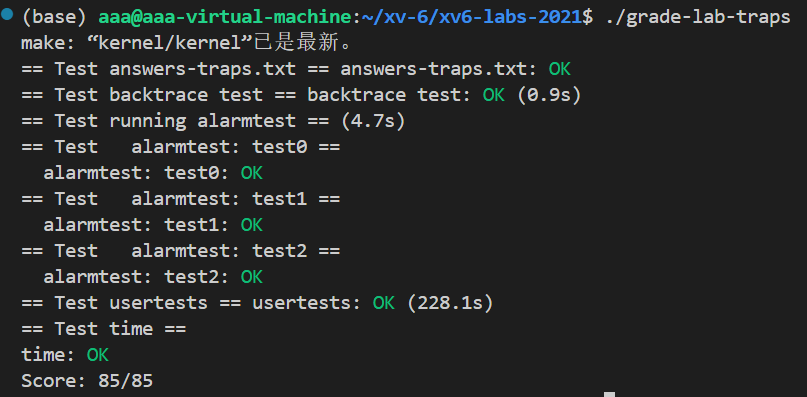
\includegraphics[width=\linewidth]{pics/traps评测结果.png}
    \caption{评测结果}
    \label{fig:traps}
\end{figure}


\subsection{实验小结}
本次实验通过实现系统调用和陷阱机制,深入理解了操作系统的核心功能。

这些操作增强了我对计算机体系结构、异常处理机制和系统调用流程的理解。通过实际编写和测试系统调用,我更好地理解了用户态和内核态之间的交互机制,以及系统调用是如何在硬件和操作系统之间传递控制权的。实现陷阱机制和backtrace功能,使我熟悉了如何捕获和处理异常,以及如何在错误发生时进行有效的调试和错误定位。添加定时提醒功能(sigalarm)使我了解了如何在操作系统中实现高级特性,从而提高系统的可用性和可靠性。通过设置定时器,可以更好地理解系统中断。

总的来说,本次实验不仅增强了我对操作系统原理的理解,还提升了我在实际系统开发中的调试和错误处理能力。
